\documentclass{article}

\usepackage{times}
\usepackage[letterpaper, margin=1in]{geometry}
\usepackage{listings}
\usepackage[T1]{fontenc} % fonts in T1 seem to look nicer, esp for listings
\usepackage{txfonts}  % apparently needed to fixup the formatting of lstlistings
\usepackage[protrusion=true,expansion=true]{microtype} % improves text layout
\usepackage{multicol}
\usepackage{xspace}
\usepackage{color}
\usepackage{url}
\usepackage{graphicx}

% tldrs
\usepackage{wrapfig}
\usepackage{tcolorbox}
\usepackage{lipsum}
\newenvironment{tldr}[1][r]
  {\wrapfigure{#1}{0.33\textwidth}\tcolorbox}
  {\endtcolorbox\endwrapfigure}

\lstset{
basicstyle=\ttfamily\footnotesize,       % the size of the fonts that are used for the code
numbers=left,                   % where to put the line-numbers
numberstyle=\ttfamily,      % the size of the fonts that are used for the line-numbers
%aboveskip=0pt,
%belowskip=0pt,
stepnumber=1,                   % the step between two line-numbers. If it is 1 each line will be numbered
%numbersep=10pt,                  % how far the line-numbers are from the code
breakindent=0pt,
firstnumber=1,
%backgroundcolor=\color{white},  % choose the background color. You must add \usepackage{color}
showspaces=false,               % show spaces adding particular underscores
showstringspaces=false,         % underline spaces within strings
showtabs=false,                 % show tabs within strings adding particular underscores
frame=leftline,
tabsize=2,  		% sets default tabsize to 2 spaces
captionpos=b,   		% sets the caption-position to bottom
breaklines=true,    	% sets automatic line breaking
breakatwhitespace=true,    % sets if automatic breaks should only happen at whitespace
columns=fixed,
basewidth=0.52em,
xleftmargin=6mm,
xrightmargin=0mm,
numberblanklines=false,
language=Scala,
escapeinside={(*}{*)}
}
% \lstset{
% framexleftmargin=15pt,
% basicstyle=\footnotesize
% }

\newcommand{\vml}{VML\xspace}

\newcommand{\core}{core\xspace}
\newcommand{\mantle}{mantle\xspace}
\newcommand{\crust}{crust\xspace}
\newcommand{\Core}{Core\xspace}
\newcommand{\Mantle}{Mantle\xspace}
\newcommand{\Crust}{Crust\xspace}

\newcommand{\version}{\texttt{Version}\xspace}
\newcommand{\richversion}{\texttt{RichVersion}\xspace}
\newcommand{\thing}{\texttt{Thing}\xspace}
\newcommand{\node}{\texttt{Node}\xspace}
\newcommand{\edge}{\texttt{Edge}\xspace}
\newcommand{\structure}{\texttt{Structure}\xspace}
\newcommand{\graph}{\texttt{Graph}\xspace}
\newcommand{\TVID}{\texttt{TVID}\xspace}
\newcommand{\tag}{\texttt{Tag}\xspace}
\newcommand{\uri}{\texttt{URI}\xspace}

\newcommand{\versiongraph}{version graph\xspace}
\newcommand{\modelgraph}{model graph\xspace}
\newcommand{\lineagegraph}{lineage graph\xspace}
\newcommand{\versiongraphs}{version graphs\xspace}
\newcommand{\modelgraphs}{model graphs\xspace}
\newcommand{\lineagegraphs}{lineage graphs\xspace}
\newcommand{\groundwire}{GroundWire\xspace}


\newcommand{\jmh}[1]{{\textcolor{red}{#1---jmh}}}
\newcommand{\vikram}[1]{{\textcolor{blue}{#1---vikram}}}

\newcommand{\eat}[1]{}

\author{
Vikram Sreekanti \hspace{2in}
Joseph M. Hellerstein\\
       {\scriptsize \{vikrams, hellerstein\}@berkeley.edu}
}
\title{Common Ground: A Metamodel for Shared Metadata Services}
\date{}

\begin{document}
\maketitle

\begin{abstract}
This document presents the metamodel for the Ground metadata service, which we call Common Ground.  Common Ground presents users with an interleaved graph model: \emph{\versiongraphs} capture metadata evolution, \emph{\modelgraphs} enable a diverse range of metadata structures and semantics, and \emph{\lineagegraphs} capture behaviors over data. 

These user-facing graph abstractions roughly correspond to concentric layers of the metamodel. The \emph{\core} of Common Ground presents the underlying abstraction of versioned objects; though it is not exposed above Ground, it is inherited by all the remaining components of the metamodel.  The \emph{\mantle} presents the foundation of the user-facing metadata modeling, a graph model that allows users to represent metadata in a wide variety of data models.  Finally, the \emph{\crust} is a layer of basic common semantic objects shared by all users, including principals, workflows and data lineage dependencies.
\end{abstract}




\section{Introduction}
\emph{Ground} is an open-source metadata service under development at UC Berkeley.  Ground is motivated by our experiences with users of open-source data processing packages like Spark, Hadoop and Jupyter, and the software vendors that provide tools and services in those ecosystems.  We have repeatedly heard requests in those communities for a flexible, vendor-neutral, open-source metadata service that can support the open source data management ecosystem, and the users and developers that have rallied around it.

This document lays out the initial design of Common Ground, the \emph{metamodel} underlying Ground that provides an abstract representation of the kinds of metadata that can be captured.  We also provide reference interfaces (traits) in Scala.
%This metamodel captures our initial design for an expressive least common denominator for metadata services, particularly in analytic environments found in modern scientific and business contexts.
Common Ground determines the basic utility of Ground's storage representation: it defines the expressivity of the metamodel, and hence scopes the class of services that can be built above Ground to support specific use cases.

\subsection{Considerations for a New Metamodel}
In most modern data management environments, data storage (the arrangement of bits in memory or on disk) is often explicitly separated from data modeling (the description of how to interpret those bits). Data can be stored with no models, to simplify data capture and support ``structure-on-read'' interpretation.  Data can also be viewed through the lenses of multiple alternative models, to support a diversity of interpretations for different use cases, often executed using different software frameworks.

In this heterogeneous environment, any metadata service must support a common metamodel that is general (to support a range of use cases) yet relatively simple and stable (to minimize disruption for the services built above).  In designing Common Ground we are inspired by Postel's Law~\cite{postel} of robustness, a tenet of Internet design philosophy:
\begin{quote}
\emph{Be conservative in what you do, be liberal in what you accept from others.}
\end{quote}
In particular, we do not want to be doctrinaire regarding a specific model of metadata, in terms of either representation or semantics.  Instead, we want to offer a unifying but flexible framework that 
%lets a variety of applications above Ground register and track their metadata with 
accommodates a diversity of metadata structures or models.  This can allow multiple applications to share the same metadata service and, over time, grow to interoperate.

\subsection{Toward Common Ground}
The Common Ground metamodel is based on an interleaved, three-layer graph structure we call a \emph{\vml graph}.  In the spirit of robustness, the central construct is simple and flexible: a \emph{\modelgraph} $M$ of nodes and edges for describing data, flexible enough to admit a diversity of traditional data models.
% (relational, entity/relationship, hierarchical, network, semi-structured, linked, etc.) 
Underneath that inventory graph is a \emph{\versiongraph} $V$, which can track a variety of models 
of revision history for individual objects and collections. Above the metadata graph is a 
\emph{\lineagegraph} $L$ used to capture the lineage of how pieces of data are derived.

This document presents an early design of Common Ground that we are using in a prototype implementation.  We expect the metamodel to evolve---quickly at first as it hones onto a good ``fit'' with a range of use cases, but hopefuly relatively rarely thereafter.  The document will be updated periodically to track the evolution of the metamodel and its use.

\begin{figure}
\centering
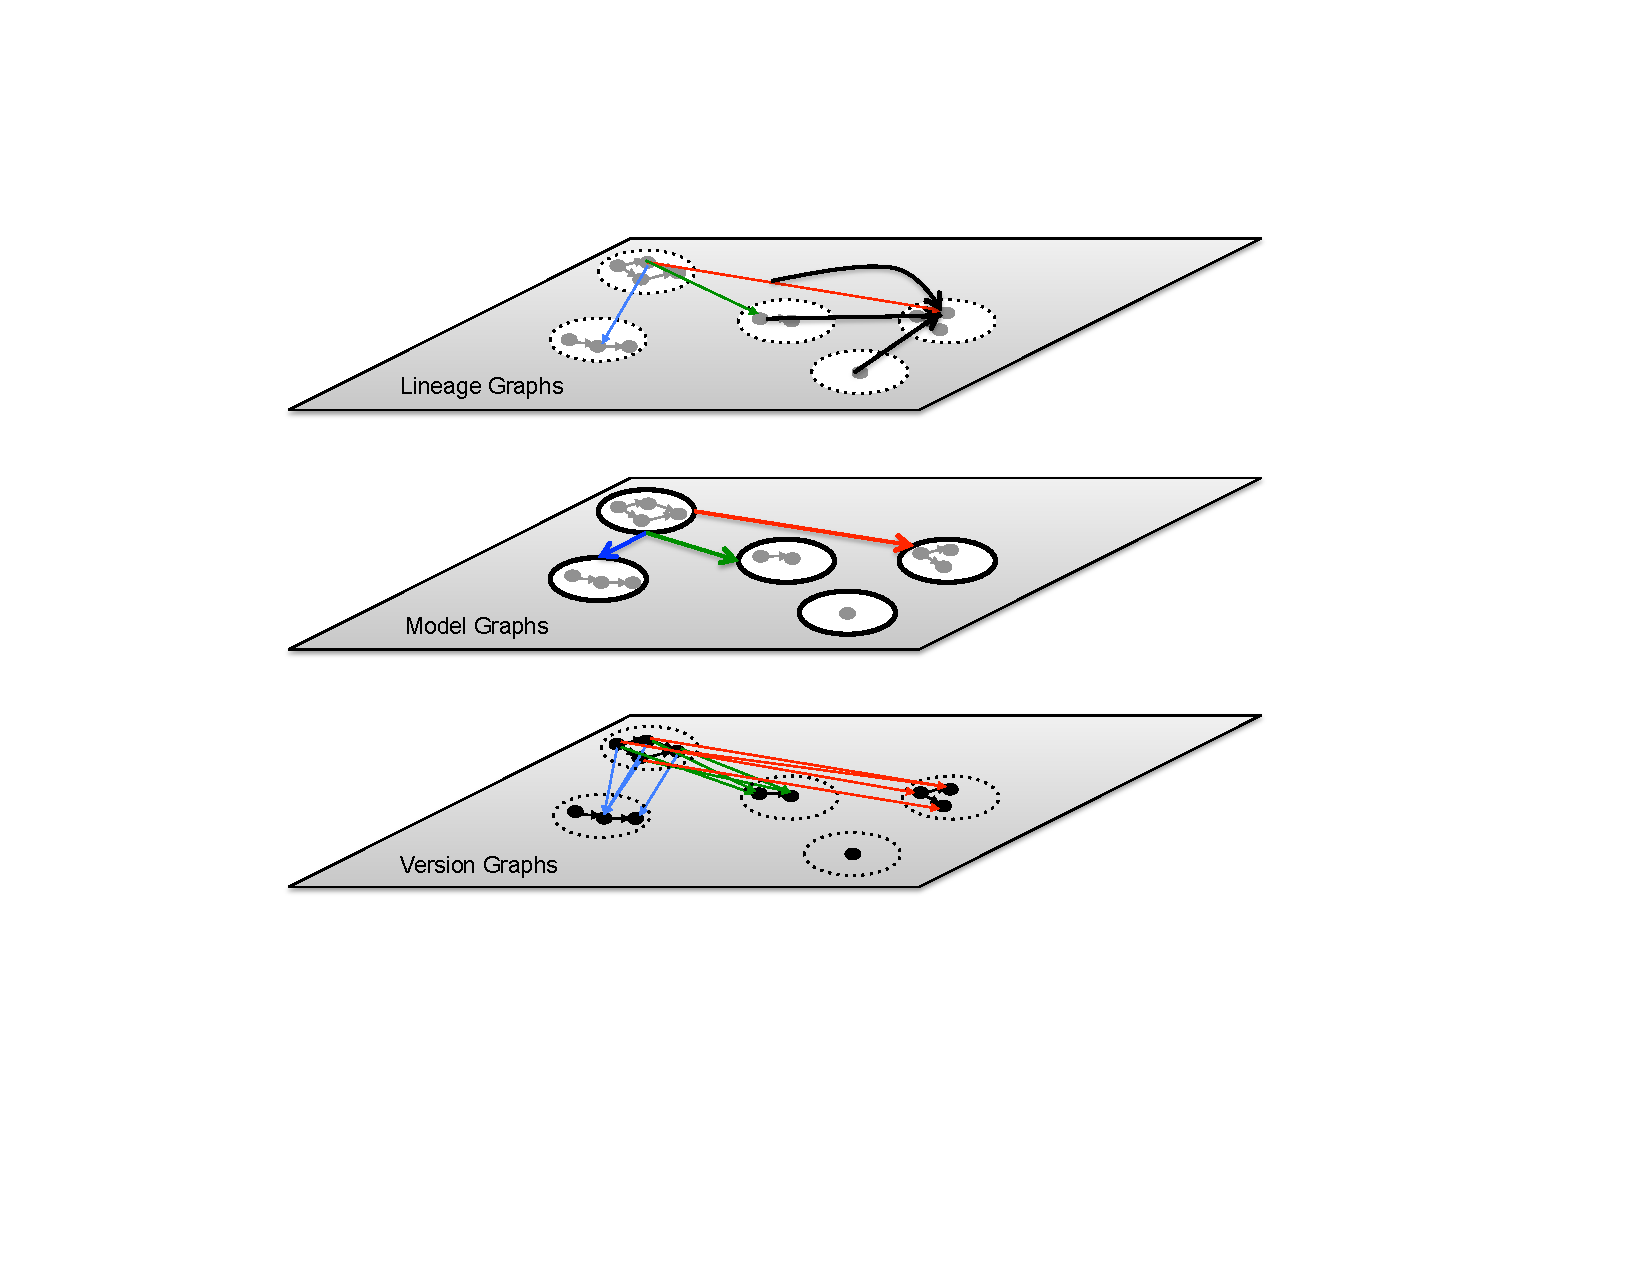
\includegraphics[width=0.75\linewidth]{layers.pdf}
\caption{The three-layered \vml model.  The central layer shows {\node}s and {\edge}s.  
Lined up below them are corresponding black \texttt{NodeVersion}s and color-coded \texttt{EdgeVersion}s.  
The black \texttt{LineageEdgeVersions} in the top layer show an example of data lineage among specific \texttt{NodeVersion}s and \texttt{EdgeVersion}s.  For simplicity, the figure omits \texttt{VersionSuccessor} relationships between different \texttt{LineageEdgeVersion}s at the top, and between \
\texttt{EdgeVersion}s in the bottom layer.}
\label{fig:layers}
\end{figure}

\subsection{Background}
The focus of this document is on the Common Ground metamodel, so we pause only briefly to review the motivations of the Ground project that drove the design of the metamodel~\cite{StrataNYC15}.  In short, they include the following list, which is intended to be suggestive but not comprehensive.
\begin{itemize}
\item {\bf Data inventory}: Like any metadata system, we want to provide facilities to store basic information about the data of interest, including how it is named, typed, structured and accessed, 
and summaries of its content.

\item {\bf Usage}:
 % Motivation: Many big data environments are designed to support analytic workloads, including both exploratory analytics (e.g., charting or ad hoc statistics), as well as production analytics workflows (e.g., log processing or model serving).  In these environments, it is useful to track
 In addition to capturing the basic intrinsic attributes of data, we also want to capture information about its usage: the way data is transformed and analyzed both by ad-hoc manual efforts and programmed workflows.  This usage information can be valuable to a number of our other goals below, some of them quite traditional (e.g. audit logs for governance), others more novel (e.g. query logs for learning statistical models of user expertise or data utility).
 %It can also enable a host of interesting new functionality, including the modeling and mining of analytic activity within an organization to improve efficiency, identify expertise, and detect institutional biases.
 %Key aspects of this use case include \emph{activity tracking}, \emph{data lineage} and \emph{.

\item {\bf Reproducibility}:
% It is well appreciated that data sets are growing and become more widely used.  Analytic methods for these data sets are becoming increasingly intricate, both in their computational goals and in the variety of tools and libraries they use to go from ``raw data'' to ``results''. Reproducibility of analytic pipelines is a critical aspect of managing this complexity.
We want to enable reproducibility of complex workflows that generate data products. As a feature, Reproducibility has many virtues.  Primarily it fosters confidence in the veracity of results from complex data processing.  Reproducibility also enables reexecution of workflows after emending the data, models or software used in a data-centric process.  This serves over time to enable ``data debugging'', ``what-if'' analysis and evolution of data interpretations.

\item {\bf Model-based interpretation}:  
%Traditionally, the word ``modeling'' has had separate meanings in the fields of databases and statistics.  The database community traditionally focused on data models and schemas (relational, hierarchical, semi-structured, etc.), as well discrete semantic models (ontologies, dictionaries); analytical software from the statistical community focus on statistical models, physical models, and the methods (learning, inference) that connect them to the consumption and production of data.
A goal of Ground is to capture models as first-class entities, and provide orthogonality between models and data.  This encompasses a breadth of database models for representation of data (e.g., relational, semistructured, linked, etc.) and mathematical models for describing and predicting the process generating the data (e.g., statistical or physical models).

\item {\bf Interoperability}: An ongoing source of frustration in data processing is the inability of tools and organizations to interoperate.
%Traditionally, interoperability was achieved via standards; this was a time-consuming and political process.  In principal, widely-adopted and open source solutions like Hadoop, Spark and Jupyter should allow interopability to occur via open source and network effects.  As certain APIs and formats become mature and widely used, they serve as centers of gravity, and many systems begin to adopt them.  We have seen some of this activity around storage formats like Avro, ORC and Parquet.
A goal of Ground is to provide an environment where data interoperability can occur de facto in an open  fashion, via open source implementations and network effects.  This is similar to the emergence of formats like Avro, ORC and Parquet for data storage, but at the higher semantic level of data modeling to capture the interpretation and use of data across users and applications.

\item {\bf Collective governance}: A common role for metadata is to help \emph{govern} the use of the data it describes.  That includes modeling principals (e.g., users, groups, roles) and rights (e.g., read, update, create, execute, grant), capturing policies to be enforced (e.g., based on attributes of principals, data contents, location, time-of-day, etc.), and auditing user behavior for post-hoc analysis.
%Traditional IT environments place the creation and management of this governance metadata in the hands of ``superusers'' of one form or another, typically IT staff.  In many analytic environments today, a different approach is preferred, which distributes this authority much more broadly and flexibly to end-users who understand the data that is arriving and the experiments being performed.  Between these poles, ``curation''is needed to help data evolve smoothly from raw materials to widely used reference.
A goal of Ground is to provide a framework for a diversity of data governance philosophies, from the top-down control seen in traditional IT environments, to emergent ``collective'' governance models that foster end-user exploratory work and Wikipedia-style community curation.
 % In those agile environments, the principals best suited to assess data are not the IT superusers, but rather the end-users who understand the data and its use deeply.  For those environments, Wikipedia is a better model than traditional IT governance structures.  In many cases, a mix of governance models emerges, to ``lock down'' data sets that are known and sensitive, while simultaneously fostering ``sandboxes'' and ``landing zones'' for more agile useage.  As data migrates from ``landing zone'' to ``lock-down'', intermediate models can be advantageous to ``curate'' data
\end{itemize}

The metamodel we describe next is intended to be a simple common denominator for all these design goals, though clearly many of these goals would need additional functionality from above-Ground layers of modeling and software.

\subsection{A Note on Implementations}
The goal of this document is to lay out a metadata model, with a focus on the \emph{logical} constructs needed to represent metadata.  Therefore our goal is to ensure that the metamodel is expressive enough to capture the kinds of metadata that need to be stored, yet sensibly constrained to be natural to adopt and interpret.  It is not our goal in this document to dictate an efficient \emph{physical implementation} of this metamodel.  Even though we present Scala traits for the metamodel to concretize our discussion, readers are cautioned not to treat these as prototypes for an implementation.

Two immediate implementation decisions are unaddressed in our specification.  The first is how to modeling one-to-many and many-to-many relationships between objects.  In our discussion we will model interfaces that allow these relationships to be represented in a manner that is natural to the discussion.  For implementations, there are a variety of choices a developer might make for performance---e.g., (de)normalization, indexing, clustering, etc.---depending on the storage medium (RAM, Flash, disk), data and workload.  A second natural question is in efficient delta encoding of versions; in our metamodel we will simply assume that versions can be treated as if fully materialized.  Again implementation choices on representation and evaluation---e.g., lazy vs. eager materialization--could be made based on storage, data and workloads.

\section{\Core Metamodel: Version Graphs}


\begin{figure}[ht]
\begin{scriptsize}
\begin{multicols}{2}
\lstinputlisting{scala/core.scala}
\end{multicols}
\end{scriptsize}
\caption{\Core metamodel in Scala.}
\label{fig:core}
\end{figure}

The \core layer of Common Ground bootstraps the representation of nearly all information in the Ground metadata service, by providing immutable objects called {\thing}s, whose evolution is captured by {\version} objects linked into a \emph{\versiongraph} abstraction.  In this section we step through the main aspects of the \core.

Versioning forms the core of Common Ground for two reasons.  First, metadata is long-lived, and provides the key to understanding the history of data and how it gets used.  Given the shrinking costs of storage and the increasing value of understanding data, we believe that metadata services are required to support complete history---for auditing, reproducibility, and debugging, among other reasons\footnote{Ground's design does not preclude the possiblity of truncating version history as a matter of system management, e.g., if storage is limited or policy dictates that certain metadata be retired.}.
Second, on a more technical note, the definition of the underlying versioning graph in Ground is the one place where we do not need (and in fact could not sensibly use) a versioned model of data.  Hence it 
makes sense as the lowest layer of the model.

Scala traits for the \core are shown in Figure~\ref{fig:core}.  We begin by discussing the \version, which is just a globally unique identifier representing an immutable version of an object.
A \texttt{VersionSuccessor} relationship is a pair of \version IDs that indicates that the
first \version is a child (``edit'') of the second \version, which immediately succeeds it.
% \jmh{N.B. We will need to
% define what ``edit'' might mean, and encompass merging as well because it's a
% DAG.}.  
Note that a \version may have many \texttt{VersionSuccessor}s, that form ``siblings'' in a partial order (a ``fork'' in history).  Similarly a single \version may be the \texttt{VersionSuccessor} of multiple ``parent'' {\version}s (a ``merge'' in history). Each version successor must link two objects from the same
subclass of \version, so a \texttt{VersionSuccessor} is a parameterized type that takes a subclass of
\version.

The \versiongraphs of the \vml are represented by the \texttt{VersionHistoryDAG}, consisting of a root $R$ (a \version) and a set of
\texttt{VersionSuccessor}s that form a DAG rooted at $R$.
%(i.e., R transitively points to all other items). 
All of the \texttt{VersionSuccessor}s in a given DAG need to link the same kind of 
{\version}s together, so the \texttt{VersionHistoryDAG} is also parameterized on a subclass of \version.

\begin{tldr}
The basic structure of the \core consists of immutable {\thing}s and a \lineagegraph of their \version history.  
\end{tldr}

The last element of our \core metamodel is the critical building block for
the rest of our metamodel: the \thing. A
\thing is an object that captures its own version history: it has a
unique ID and a \texttt{VersionHistoryDAG}. A \thing is parameterized on the subclass of
\version that it contains in its \texttt{VersionHistoryDAG}.  As we will see in the next section, most of the metamodel will use {\thing}s to capture the immutable aspects of an object, and the associated {\version}s to capture changes 
to the object.

% \jmh{Do we want an equivalent of \tag for \thing?}

The \core is not exposed to above-Ground (user-level) services; it is the root of an inheritance hierarchy that is exposed by the outer layers described below.  From this point on, when we speak of {\thing}s and {\version}s, we will actually be referring to objects in the subclasses defined below that are visible above Ground.

\section{\Mantle Metamodel: Metadata Graphs}

\begin{figure}[ht]
\begin{scriptsize}
\begin{multicols}{2}
\lstinputlisting{scala/mantle.scala}
\end{multicols}
\end{scriptsize}
\caption{\Mantle metamodel in Scala.}
\label{fig:mantle}
\end{figure}

% Our philosophy is that the metamodel should be designed in layers for
% simplicity and elegance. \core classes are shared and evolve in infrequent,
% regimented updates to maximize backwards compatibility. More detailed versions
% of the metamodel (including versions specific to use cases) are mapped onto
% simpler versions of the model. Our goal to find a balance between the
% simplicity and the expressivity of the metamodel and leave the rest up to the
% application using this metamodel.

% To illustrate this philosophy, we have developed a somewhat richer metamodel
% that can be imposed onto the aforementioned model.

The next level of Ground, the \emph{\mantle}, presents the basic metamodel exposed above Ground: notably it defines {\node}s and {\edge}s that can be collected into {\graph}s for representing metadata.  All of these objects and collections inherit from \thing, and hence are versioned.   Scala traits for the Mantle are shown in Figure~\ref{fig:mantle}.

The basic structure of the \mantle is defined by pairs of classes,
which inherit from the \core's \thing and \version classes respectively.   As a
naming convention, each subclass of \thing in the mantle has a corresponding
subclass of \version with the same name, but appended with a \texttt{Version}
suffix (e.g. \node and \texttt{NodeVersion}, \edge and \texttt{EdgeVersion},
etc.)  By inheriting from the core, all {\thing}s in a
subclass like \node contain a unique \texttt{Id} as well as a
\texttt{VersionHistoryDAG} that associates the \thing with many versions from
the associated version class.  
% In turn, all {\version}s in a subclass like
% \texttt{NodeVersion} are identified by a \texttt{TVID} (Version ID) that stores
% both the ID of the corresponding \thing , and another \texttt{VersionID}
% to distinguish the specific \version.  
% It is thus possible to determine {\thing}s
% from their {\version}s and vice versa.  
% \jmh{There is a 1-to-many constraint
% between {\thing}s and {\version}s.  Worth noting, and asserting somewhere in the
% code.} \vikram {We agreed that we didn't need actually add anything about this
% to the document, right?}

To provide customization, we want to allow {\version}s to be augmented
with both unstructured and structured information; {\version}s are
immutable, so this information has to be associated upon creation. For unstructured information, 
we define a notion of {\tag}s, in the 
form of keys with optional typed values.  Like {\version}s, {\tag}s are also immutable.
  % {\tag}s refer to the {\version} that contains them; 
  %a \tag is uniquely identified by its \version and key.  
% , a new \version subclass (e.g. \texttt{NodeVersion}) must be generated to hold the new {\tag}s, and linked as a successor into
% the \texttt{VersionHistoryDAG} of the corresponding \thing\footnote{Logically,
% the new version would likely contain a copy of all the unmodified {\tag}s
% of the preceding version as well, though in an implementation this could be
% encoded more efficiently.}.  
% We also allow {\tag}s to be associated with {\thing}s, 
% enabling users to register immutable tags that apply to all versions of a \thing.  \jmh{Need to get 
% this into the code.}  

In addition to ad-hoc {\tag}s,
{\version}s can be associated with structured information by referring to a
\texttt{StructureVersion} object. {\structure}s provide a prescribed format for {\richversion}s to follow. 
A \texttt{StructureVersion} consists of a set of key-type pairs.
Each \version that references this \texttt{StructureVersion} must have {\tag}s with the corresponding 
keys and types.


\begin{tldr}
The state of each \thing is represented by a combination of immutable properties from a \thing subclass, and {\tag}s (structured or unstructured) from the corresponding \version subclass.
The \core definitions are internal, and only exposed above Ground via inherited classes.
\end{tldr}
Up to this point we have referred to types rather loosely.  Ground currently includes 
a typical set of built-in atomic types common to most languages: booleans, characters, strings, and
numerics.  For now most of these types are being taken from Scala; we will evaluate whether additional 
atomic types (e.g. SQL's decimal type) need to be built in.  One important type that is specific to 
Ground is the Uniform Resource Identifier, or \uri.  We will describe the use of {\uri}s in more detail in the next section.  As of now we have no plans for user-defined types in Ground, though we will revisit
this decision as we progress.

We can now define {\richversion}s, which are {\version}s that can optionally be augmented with application-specific information in the form 
of optional typed {\tag}s and \texttt{StructureVersion}s.  By parameterizing on \richversion, our remaining \thing subclass are user-customizable.  The immutable aspects of objects from these subclasses are captured in a \thing subclass
(e.g. \node), and the mutable aspects in the corresponding \richversion subclass (e.g.
\texttt{NodeVersion}).  

% These basic objects are quite simple, but they can be customized by attaching
% ad hoc \texttt{Attributes} to their versions: these are key/value pairs that can
% be attached to a specific \version. \jmh{Not clear from the Scala how you get attributes of a \thing!}
% Optionally, {\version}s can also have a \texttt{Structure} that they impose: a set of attributes
% that they must contain.
% This more complex
% metamodel will simply be a composition of the building blocks we highlighted.
% The \mantle serves as the basis for increasingly rich, use-case specific forms of metadata that can be structured on top of this intermediate
% metamodel, benefiting both from the versioning embedded in the \core, and
% the typed graphical structure of the \mantle.


As mentioned above, the critical subclasses are \node and
\texttt{NodeVersion}, \edge and \texttt{EdgeVersion} and \graph and
\texttt{GraphVersion}.  The \node, \edge and \graph classes are very simple, containing
no more information than the \thing superclass provides.  Likewise the 
\texttt{NodeVersion} class contains the same information as the \richversion class, albeit in
a publicly visible interface.
% However, both the
% \texttt{NodeVersion} and \texttt{EdgeVersion} classes augment their \version
% superclass with an optional reference to a \texttt{StructureVersion} (that we
% will describe shortly) to represent a required structure for the version.
The \texttt{EdgeVersion} subclass carries a bit more information than its parent class, 
by providing the two \texttt{NodeVersion} endpoints of the \texttt{EdgeVersion}.
\texttt{GraphVersion}s are more interesting: they enable access to a set 
of \texttt{EdgeVersion}s.  Like other properties of a \version, that set is immutable.  Hence a new 
\texttt{GraphVersion} needs to be generated to capture the \graph being modified by insertion,
deletion, or update of an existing \texttt{EdgeVersion}.

  % Working through the definitions of
% Figure~\ref{mantle} you can see straightforward definitions of \texttt{Set}s
% and \texttt{SetVersion}s, which inherit from \thing and \version.  The \graph
% class inherits from \texttt{Set} without modification; the
% \texttt{GraphVersion} class extends \texttt{SetVersion}.

  % \jmh{For symmetry, we should probably rename \version to Version, and \thing to something else like a Thing.} \jmh{We need a naming convention for these things to avoid the goo of discussing objects and versions in an ad hoc way.}


% In the \mantle metamodel, we have a number of objects that each extend the
% \texttt{VersionedItem}. For each of object (say) ``\texttt{Foo}'', there is a
% corresponding ``\texttt{FooVersion}''
% class.
% These classes extend the \version class and compose the \texttt{VersionHistoryDAG}
% for the objects that they represent.

% We also have collections of {\node}s and {\edge}s. In order to illustrate the
% design of these collections, let's consider the example of a \graph, which is
% represented simply by a set of {\edge}s. A \graph, just like all the other objects
% in the \mantle, is a \thing. 
% Versions are more complex for a collection type like {\graph} than for scalar types like \node or \edge.
% A \graph's version can change in two different ways. The first is simple: when you add or delete an \edge from the \graph, you implicitly create a new
% version of the \graph container. The
% second is if the {\edge}s themselves are modified---in particular, when the
% endpoints of the \edge change, even though the identity of the edge may not\footnote{As a motivating example, consider an ``ownership'' \edge that represents the current owner of a file.  This fact does not change identity, it just links to a different principal as the owner, allowing us to track the ownership of that file over time.}. This second case poses an interesting challenge
% in terms of correctly propagating versioning changes. In order to solve this
% problem, every \thing has the capability of being ``watched''. That is,
% every object has a list of subscribers to which it publishes updates.
% In Ground, a \graph
% watches every one of its {\edge}s, and if an \edge is modified, then the \graph
% will also create a new version of itself with this \edge.  \jmh{This feels imperative.  Instead, how about a declarative description of a constraint: the version of a Graph relates in some way to the most recent version of any Edge it contains.  You could probably leave out the description of how this is achieved
% entirely.} \vikram{Maybe I'm not understanding what you mean by declarative
% here, but if you read up until the sentence that ends with "the identity of the
% edge may not, I think it describes the ways in which the identity of a graph
% depends on its edges. Beyond that, if we want to leave out a description of how
% we're accomplishing this, then we can just cut out everything after that,
% right? Or is there something else missing?}

\begin{tldr}
The \mantle provides the metamodel for above-Ground services: versioned {\graph}s formed
by {\node}s and {\edge}s.  This captures the salient aspects of most common data models.
\end{tldr}

Lastly, we have a notion of \texttt{ExternalThing}s. \texttt {ExternalVersion}s 
contain a required \uri reference to some external source, along with required timestamps, 
optional \texttt{cachedValue}s, and parameters for accessing the
reference (e.g., port, protocol, etc.) \texttt{ExternalThing}s have an \texttt{isUnchanging}
flag, which, if enabled, is an indication that the external resource is expected to be
immutable, and there should only be one \texttt{ExternalVersion} associated.
Note that this is advisory; if the actual reference changes, Ground will not be aware.

\begin{figure}
\centering
\begin{minipage}{0.4\textwidth}
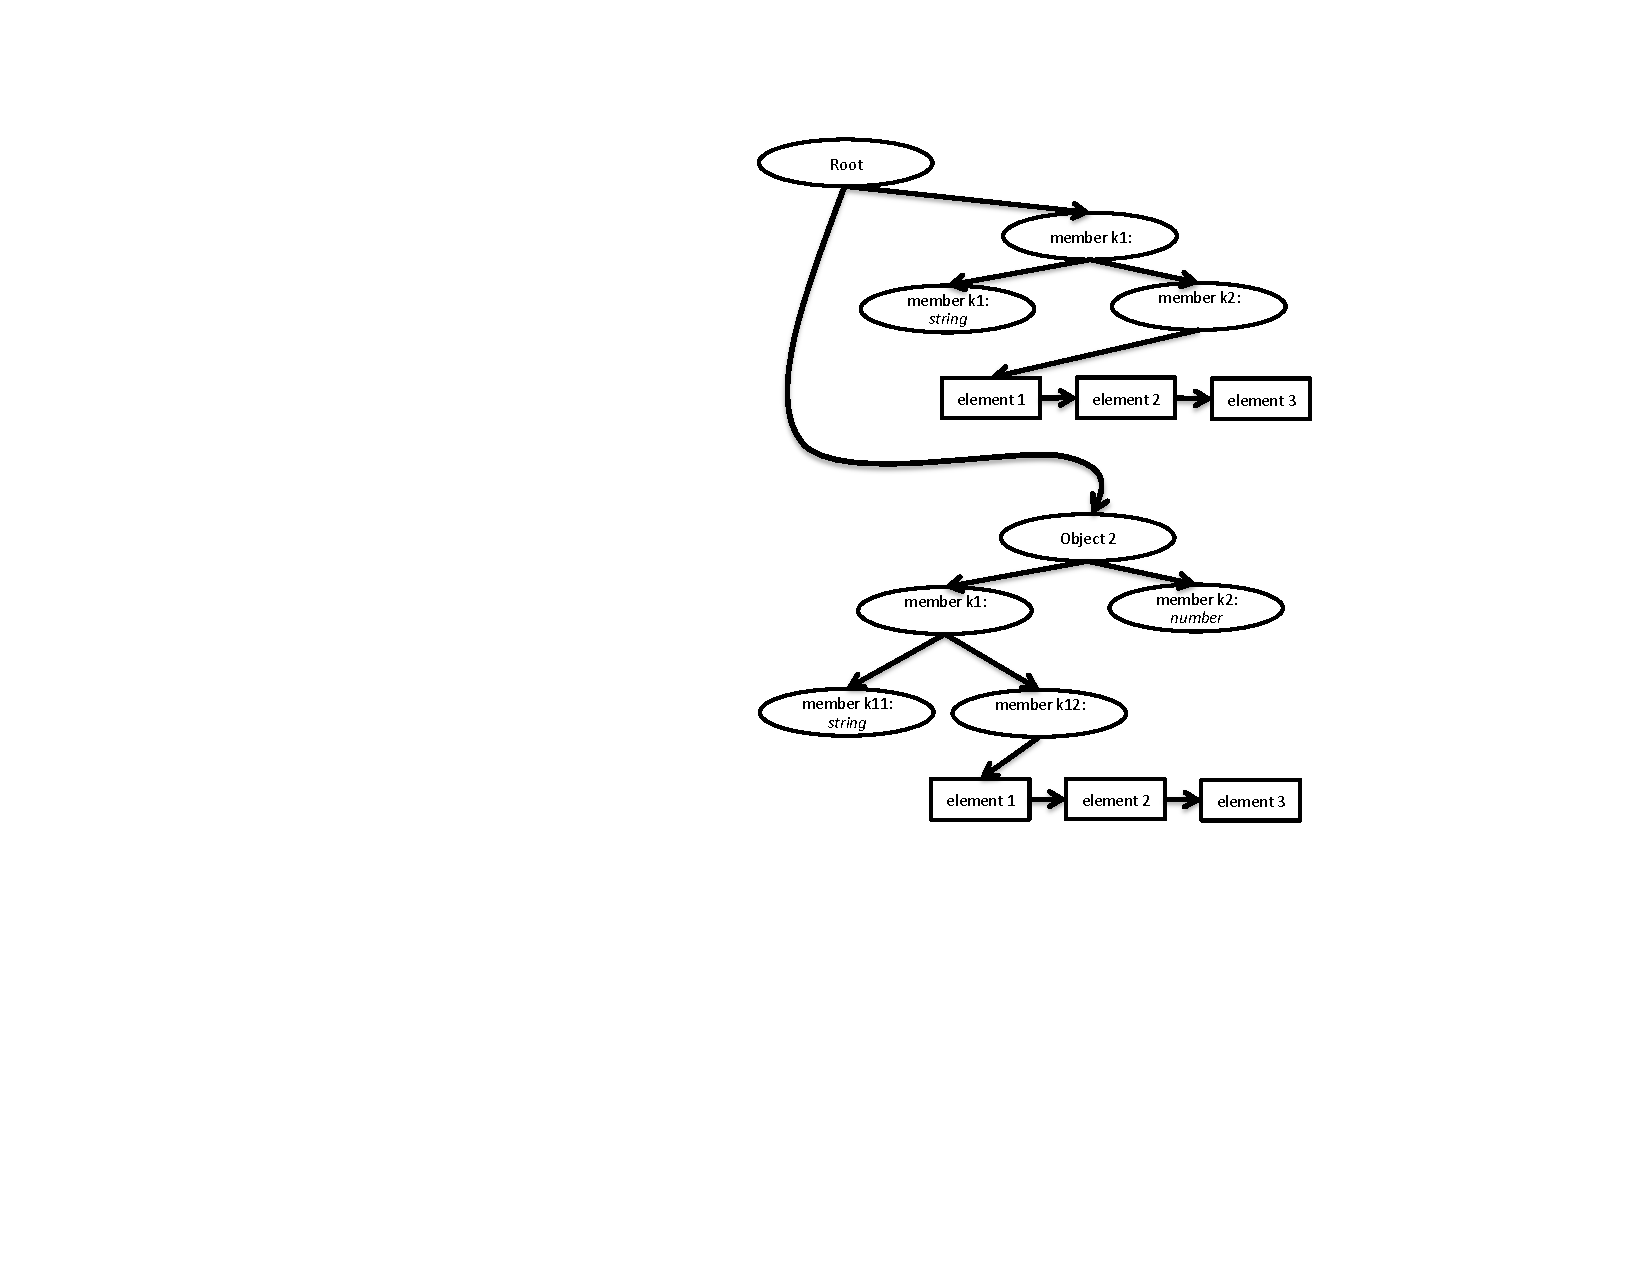
\includegraphics[height=2in]{json.pdf}
\caption{A JSON document represented as a graph.  Note the nesting of JSON objects (key-value collections) in a tree shape of oval nodes, and lists as chains of rectangular nodes.}
\label{fig:json}
\end{minipage}
\hspace{0.1\textwidth}
\begin{minipage}{0.4\textwidth}
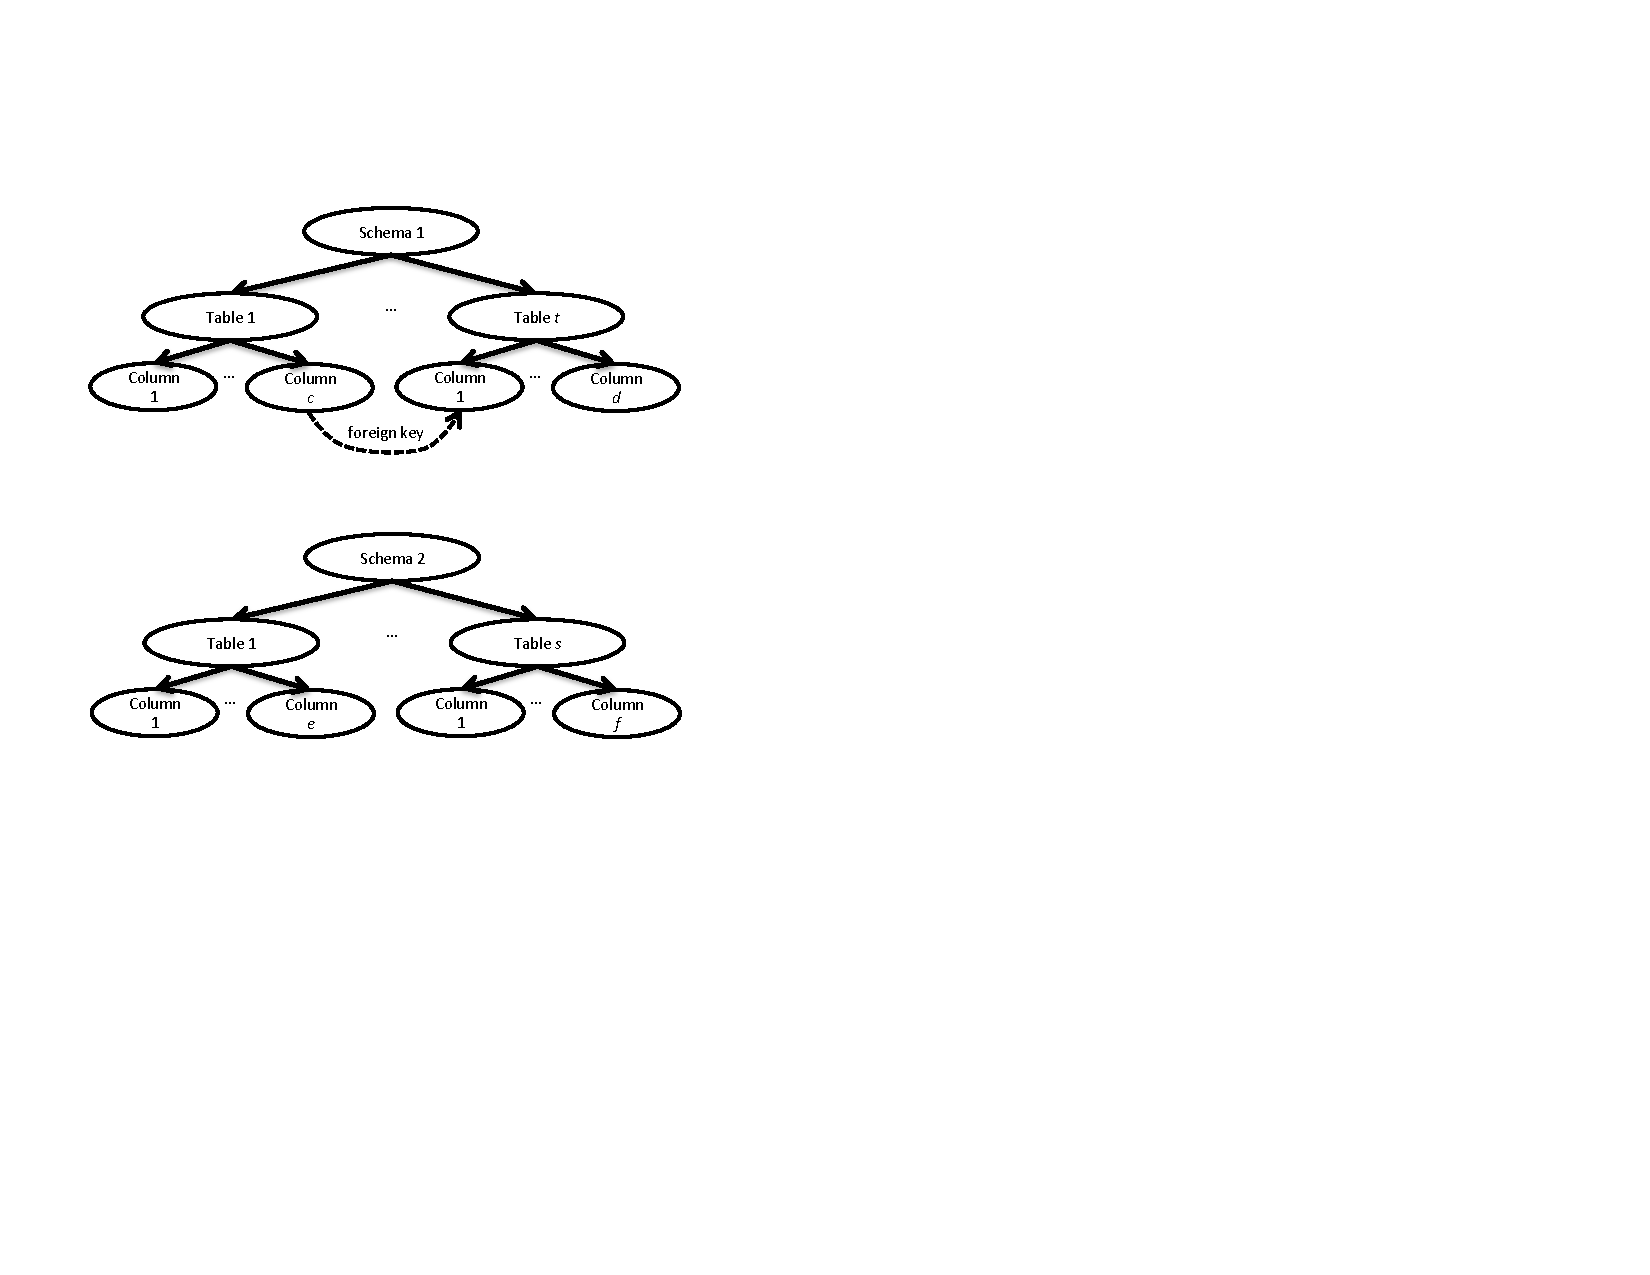
\includegraphics[height=2in]{relational.pdf}
\caption{A relational database with two schemas, represented as a graph.  Note the fixed schemas$\rightarrow$tables$\rightarrow$columns structure, and
the ad hoc foreign key references at the leaves.}
\label{fig:relational}
\end{minipage}
\end{figure}


The \mantle uses a graph abstraction for data modeling because it is extremely general, and allows for metadata to be represented in a variety of 
data models.  Unstructured data models like JSON and XML 
are very typically represented as flexible trees or graphs (Figure~\ref{fig:json}).  
Structured data models like relational and entity-relationship can be represented as graphs as well, often
with constraints on the shapes that the graphs can take on (Figure~\ref{fig:relational}).  Ground's \mantle allows diverse models
of metadata to coexist in a single metadata store, and be integrated over time.

In summary, the \mantle provides a public, above-Ground interface for building application-specific 
abstractions by customizing the optional and structured tags of nodes and edges, and laying them out in versioned graphs. 



\section{\Crust Metamodel: Provenance Graphs}

\begin{figure}[ht]
\begin{scriptsize}
\begin{multicols}{2}
\lstinputlisting{scala/crust.scala}
\end{multicols}
\end{scriptsize}
\caption{\Crust metamodel in Scala.}
\label{fig:crust}
\end{figure}
The goal of the \crust is to capture a \emph{provenance graph} in the form of
\texttt{LineageEdge}s.  To facilitate data lineage, Common Ground depends on
a notion of \texttt{Principals} and \texttt{Workflow}s that we define first.  These
are in some sense the first ``semantic'' objects in Common Ground; we believe they are fundamental
to any metadata system as parameters of provenance.

\texttt{Principal}s are key concepts for capturing the actors that work with data, particularly in support of data governance. \texttt{Principal}s are
the Common Ground representation for notions such as users, groups, and roles.
\texttt{Principal}s are particularly important
because they can be used in both auditing and
in enforcement of policies like access control.
% Note that \texttt{Principal}s
% are {\node}s, and built while access rights and group membership can be represented as {\edge}s.
% {\structure}s would be particularly useful here because users would
% have some set of required information based on the identity \& authentication
% schemes being used. 
\texttt{Principals} are integral to data lineage because
they capture responsibility for creating, modifying and accessing data---supporting
both in-line enforcement and off-line auditing of behavior.

\begin{tldr}
The purpose of the \crust is to capture semantic notions that are common across all use cases.  Currently this consists only of principals, workflows and the \lineagegraph of data dependencies.
\end{tldr}

The second concept that we believe is common is \emph{workflow specification}.
This sort of metadata is very important to Reproducibility and Usage tracking use cases.
Workflows are representable in terms of the graph
structure of the \mantle, but we believe they merit being
first-class citizens in the \crust of the Ground metamodel. These
\texttt{Workflow}s,
which are versioned, can explain what data was transformed, how it was
transformed, and what the result of that transformation was. \texttt{Workflow}s
can either be a sequence of \textit{ad hoc}, exploratory actions or a
pre-defined set of actions.

Finally we are ready to define data lineage.  In Ground, lineage
is captured as a relationship between two {\version}s, the second of which is derived from the
first. This relationship is due to some process, either computational
(workflows) or manual (via some principal). Basic \texttt{EdgeVersion}s as described
in the \mantle cannot contain references, nor can they have other {EdgeVersion}s as endpoints.  
So we introduce \texttt{LineageEdge}s, which are parameterized by the subclass of \richversion at their
endpoints, and which contain 
optional references to \texttt{Workflow} and \texttt{Principal} nodes.

\section{\groundwire: User-Defined Models Above Ground}
The three layers of the Ground metamodel are intended to be common to all uses of the service.  We 
showed Scala traits for this metamodel as a concrete example.  However, we expect users of the Ground
service to interact with it via a language-agnostic REST API called \groundwire.  Users can define their own
customization of the Ground metamodel by declaring custom {\node}s, {\edge}s, {\structure}s and {\tag}s.  
These can be packaged into libraries for common cases (e.g. a library for representing
relational database catalogs, or a library for representing JSON documents).  These libraries can 
be independent of each other, separately ``orbiting'' the unified Ground model.  

The API for \groundwire is the subject of a separate document.

\section{Design Validation}
We want to ensure that our metamodel is expressive enough to cover a diversity of common use cases that we expect in the open source data ecosystem today.  
To that end, we intend to look at a number of use cases and make sure that each layer of our metamodel is sufficiently expressive. 


\begin{itemize}
\item \versiongraph use cases: git, Wikipedia edit history

\item \modelgraph use cases: Hive Catalog, herd, Wikipedia?

\item \lineagegraph use cases: Spark, Jupyter
\end{itemize}

Beyond expressiveness, validating the design of a metamodel becomes a more subjective exercise.  For example, binary strings offer very general expressivity, but are unattractive from usability and interpretability perspectives.  An ongoing challenge for the work will be to find metrics for evaluating and tuning the ``fitness'' of the metamodel for typical use.  One goal is to try and capture metadata in a manner that is ``organic'' to its native format.  As a counter-example, taking a JSON document and normalizing it into a relational scheme is not ``organic''. A related goal in this regard is to ensure that a heterogenous mix of metadata can be kept together and rationalized/integrated incrementally over time.

We view this an evolving aspect of our design process.


\eat{
\section{Discussion: \vml Graphs}

\subsection{Extensible Version Graphs}
Discuss the extensibility here.  

Individual rooted object DAGs are good enough: no cycles, and the root can be a NULL entry (just for reference) if you don't like rootedness.

Versioned collections.  Focus on sets, insertion, modification, deletion.  Note how element versioning affects set versioning. A design space opens up: from full combinatorial branching, to more constrained models including Git and something causal like vector clocks.

\subsection{Model-Agnostic Inventory}
Show the way that many data models map into nodes+edges.  Relational, semistructured (e.g. JSON), entity-relationship, RDF triples.  Pictures will be worth 1000 words here.

\subsection{Lineage Graphs}
Note how lineage `tunnels through' the {\thing}s down to {\version}s.  We know that Lineage on {\thing}s wouldn't make sense.  But what does it mean for the {\thing}s that they have {\version}s that share a Lineage relationship?  Does the Lineage Graph in some way enrich the \thing graph? 

\subsection{Why three layers?}  
Argue (topologically?) that no 1-layer or 2-layer graph could capture the structures we want.
}

\section{Example Scenario: Course Management Metadata}
\eat{

As an illustrative example, we will discuss course management for the
undergraduate databases course at U.C. Berkeley. Handling the metadata for the
course requires interfacing with and managing data from multiple systems: the
Berkeley campus authentication system, the EECS department's identity system, and
github. This example is particularly suited for the data usage and governance
use cases. This represents the complex interaction of many systems, often held
together by Python or shell scripts, similar to common real-world use cases.

For the purposes of this course, we will have three logical objects: Students,
Assignments, and Submissions (of Assignments by Students). Our very simple
metamodel for the course can easily be imposed upon on the Ground model.
Students and Assingments are {\node}s while Submissions are {\edge}s.
Submissions connect versions of Students to versions of Assignments.
\vikram{Should we mention constraints here? e.g., Submission must always be on
the latest version of an assignment. We haven't mentioned it anywhere in the
doc, but I remember that we agreed that it was something we should support.}

Another integral part of the course metadata is workflow specification. An
example workflow for the course would be running an autograder test suite on a
Submission, writing the Student's grade into a CSV, emailing the Student their
results, and running the Submission through anti-cheating software like MOSS.
Such a workflow would be created for each assignment, where the main piece that
would vary is the autograder suite. It will be triggered by a Github webhook
every time a Student pushes their code to a certain branch on Github.

Capturing this metadata would also allow us to understand more interesting
things about our assignments. For example, if most students are not passing
most of the autograder tests the night before the assignment deadline, we might
be able to infer that the assignment was inordinately difficult. Conversely, if
we might see that all the students are passing every autograder test on their
first submission, the assignment was far too easy.
}
\section{Example Scenario: Scientific Experiment Management}

\bibliographystyle{abbrv}
\bibliography{metamodel}

\end{document}
